\chapter{Detailed design}

In this chapter, every single class is described in terms of interface and
functionality. Because of the fairly dynamic character of this project -- new
ideas come and go -- this chapter will not be finished until the end of the
project and will probably change regularly.

\section{Files and directories}

All source code will be in the directory \texttt{src/}. All classes are in the
package \texttt{amber} or in a subpackage thereof. The Psyclone specification
file \texttt{psySpec.xml} is found in \texttt{data/}. External libraries that
are redistributed with \Amber\ are in \texttt{lib/}. The source of this
document, the traineeship report and the website are located in
\texttt{documentation/}.

The application is built using Apache
Ant\footnote{\url{http://ant.apache.org/}} and it can be imported into
Eclipse\footnote{\url{http://www.eclipse.org/}}. It requires Java SDK version
1.5 or greater.

\section{Crawler module}

\begin{figure}
  \centering
  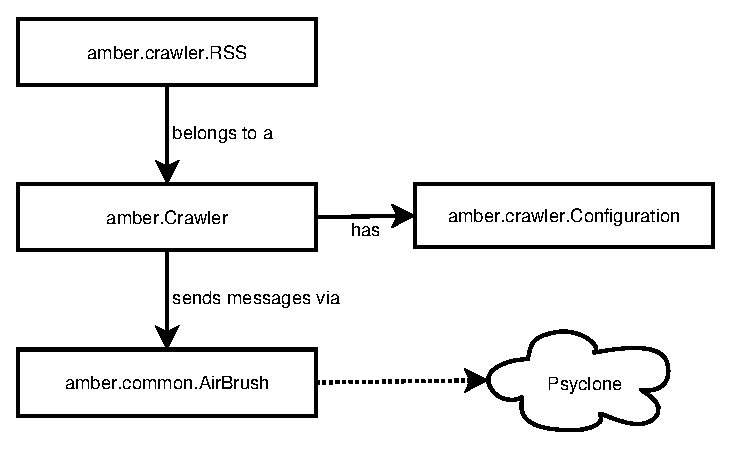
\includegraphics{image/crawler}
  \caption{
    Diagram of the design of the Crawler, the names are Java classnames
  }
\end{figure}


\section{Sieve module}

\section{ShowOff module}

\begin{figure}
  \centering
  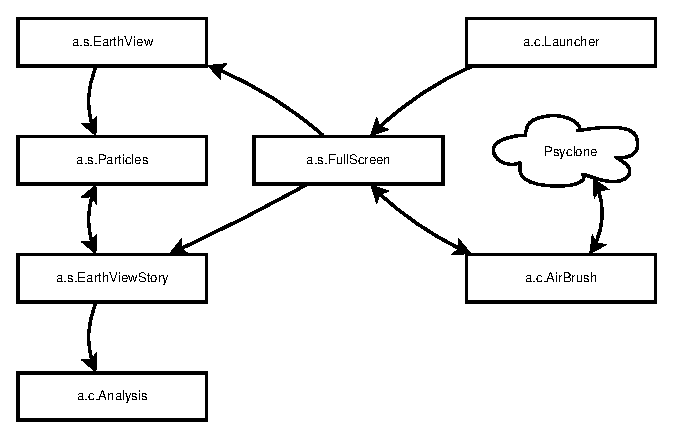
\includegraphics{image/showoff-fullscreen}
  \caption{
    Diagram of the design of the full screen ShowOff module, the names are
    abbreviated Java classnames
  }
\end{figure}

